\documentclass[11pt,a4paper]{article}
\usepackage[T1]{fontenc}
\usepackage[utf8]{inputenc}
\usepackage{lmodern}
\usepackage{microtype}
\usepackage[margin=2.6cm]{geometry}
\usepackage{setspace}
\usepackage{graphicx}
\usepackage{booktabs}
\usepackage{array}
\newcolumntype{L}[1]{>{\raggedright\arraybackslash}p{#1}}
\usepackage[font=small,labelfont=bf]{caption}
\usepackage{float}
\usepackage{amsmath,amssymb}
\usepackage{enumitem}
\usepackage{xcolor}
\usepackage[authoryear,round]{natbib}
\usepackage{titlesec}
\usepackage{fancyhdr}
\usepackage[hidelinks]{hyperref}

\definecolor{edition}{gray}{0.94}
\setstretch{1.15}
\setlist{itemsep=2pt,topsep=4pt}
\titleformat{\section}{\large\bfseries}{\thesection}{0.8em}{}
\titleformat{\subsection}{\normalsize\bfseries}{\thesubsection}{0.8em}{}
\pagestyle{fancy}
\fancyhf{}
\fancyhead[L]{\small Simons --- Mirrors and Markets, revised edition (2026)}
\fancyhead[R]{\small\thepage}
\renewcommand{\headrulewidth}{0.3pt}

\begin{document}

\begin{titlepage}
\centering
\vspace*{2.5cm}
{\small NEOMA Business School --- M.Sc Finance \& Big Data\par}
\vspace{1.8cm}
{\LARGE\bfseries Mirrors and Markets\par}
\vspace{0.5cm}
{\large Reflexivity evidence of retail traders' influence in meme stocks\par}
\vspace{1.2cm}
{\large\itshape Revised edition, 2026\par}
\vspace{2cm}
{\Large Yann Simons\par}
\vfill
\begin{minipage}{0.86\textwidth}
\small
Revised edition of the M.Sc dissertation submitted to NEOMA Business School on
31 August 2024 (dissertation supervisor: Gabriel Giménez-Roche). The original
version is kept unchanged in the same repository (\texttt{dissertation/}). This
edition keeps the research question, the hypotheses, the case study and the data
sources of the original; it corrects the data construction and the econometric
specification, and re-runs the analysis. All results reported here are produced
by the script \texttt{revised\_analysis.py} distributed with this document.
\end{minipage}
\vspace{1.5cm}
\end{titlepage}

\begin{abstract}
\noindent
This dissertation asks whether George Soros's theory of reflexivity and Reddit
sentiment can explain the price movements of GameStop (GME), the emblematic meme
stock, and whether retail trading activity amplifies them. The 2024 edition
reported a strong negative correlation between sentiment and price ($-0.897$)
and a regression explaining 82\% of the price level. This revised edition shows
that these results are artefacts: the sentiment data only start in January 2021,
and the whole of 2020 --- half of the sample --- had been filled with the score of
the first two posts available. Re-estimated on the period actually covered by the
data (5 January -- 26 August 2021, 151 trading sessions), with returns instead of
price levels, robust standard errors and tests in both directions, the evidence
is much narrower. Daily sentiment does not move with same-day returns, returns do
not feed back into sentiment, and wavelet coherence between the two is no higher
than chance. Lagged sentiment and lagged attention (the number of posts) do
predict lower next-day returns, and attention predicts volatility, but only
because of the January 2021 short squeeze; outside the squeeze window none of
these relationships survives. Trading volume is the most robust companion of
GME returns. The reflexive loop described in the 2024 edition is not visible in
daily Reddit data; if it exists, it operated during a few weeks of extreme
attention.

\medskip\noindent
\textbf{Keywords:} meme stocks, GameStop, reflexivity, investor sentiment, retail
attention, Reddit, Granger causality, wavelet coherence.
\end{abstract}

\section*{About this edition}
\addcontentsline{toc}{section}{About this edition}

\noindent\colorbox{edition}{\begin{minipage}{0.97\textwidth}\small
\vspace{4pt}
\textbf{What has not changed.} The research question, the three hypotheses, the
GameStop case study and the data sources: Yahoo Finance for GME and the VIX, and
the \emph{GameStop Reddit Dataset} \citep{han2023} for sentiment, whose scores are
VADER compound scores of post titles \citep{hutto2014}.

\smallskip
\textbf{What has changed.} (i) The 2024 regression is replicated exactly, and the
reasons why it cannot be interpreted are documented (Section~\ref{sec:replication}).
(ii) Sentiment is aggregated to trading sessions and the sample is restricted to
the days actually covered by the Reddit data. (iii) All models use stationary
variables (returns, changes in volume and VIX), heteroskedasticity- and
autocorrelation-robust standard errors and multicollinearity checks. (iv) The
leading-indicator and feedback claims are tested with Granger causality in both
directions and with wavelet coherence including Monte Carlo significance.
(v) Robustness checks exclude the January 2021 short squeeze. (vi) The text and
the reference list have been corrected.
\vspace{4pt}
\end{minipage}}

\bigskip
{\setcounter{tocdepth}{1}\small\tableofcontents}

\subsection*{Erratum to the 2024 edition}

\begin{small}
\begin{tabular}{@{}L{0.46\textwidth}L{0.50\textwidth}@{}}
\toprule
2024 edition & Correction \\
\midrule
Sentiment ``from January 2020 to December 2021''. &
The Reddit data start on 4 January 2021. In the 2024 sample, 253 of 504 sessions
(50\%) --- all of 2020 --- carry the score of the two posts of 4 January 2021
(0.989), copied backwards by a back-fill. \\[2pt]
Sentiment median and upper quartile of 0.989. &
Both are the back-filled value. Over the days actually observed, daily
sentiment averages 0.145 with a standard deviation of 0.05. \\[2pt]
Correlation of $-0.897$ between sentiment and price. &
Created by the back-fill (high constant sentiment in 2020, when the price was
low). On observed days the correlation with the price level is $-0.18$, and with
returns it is close to zero. \\[2pt]
OLS of the price level on volume, sentiment and VIX, $R^2=0.82$. &
The price level is non-stationary (ADF $p=0.85$); a level regression with an
imputed regressor cannot be read as evidence of influence. The condition number
of $2.7\times10^{8}$ comes mostly from unscaled volume. \\[2pt]
A negative sentiment coefficient described as ``heightened positive sentiment
leads to price surges''. &
A negative coefficient means the opposite; no leading relationship was tested. \\[2pt]
Sentiment averaged over four subreddits. &
The r/Superstonk file contains no sentiment score; three subreddits are used. \\[2pt]
Wavelet coherence heatmap (coherence 0--0.54). &
The preserved code computes a single correlation coefficient, not a coherence;
the heatmap cannot be reproduced. Coherence is re-estimated with significance
testing (Section~\ref{sec:wavelet}). \\[2pt]
Data limits not discussed. &
The r/GME file is truncated at 999{,}999 posts (it ends on 26 August 2021),
dates 603{,}691 posts (60\% of the file) on 16 March 2021 and has no posts on
18--26 March. \\
\bottomrule
\end{tabular}
\end{small}

\bigskip

\section{Introduction}

Meme stocks have become one of the most visible anomalies of post-Covid markets.
In January 2021, GameStop --- a struggling video-game retailer --- saw its share
price multiply roughly twenty-fold in a few weeks, pushed by retail investors
coordinating on Reddit forums such as r/WallStreetBets against hedge funds holding
large short positions. On 28 January 2021, several retail brokers, including
Robinhood, restricted purchases of the stock, and the price collapsed. The episode
became a symbol of the new influence of retail traders and of social media on
price formation.

My interest in the subject comes from my own trading experience: I traded GME and
AMC at the time, and I wanted to understand what had really driven these moves.
The theoretical lens is George Soros's theory of reflexivity
\citep{soros1987,soros1998}: market participants' perceptions influence prices,
and prices in turn reshape perceptions and fundamentals, creating feedback loops
that push prices away from equilibrium. Meme stocks seem to offer an ideal
laboratory for this idea, since retail investors' beliefs are expressed publicly
and in real time on social media.

This dissertation therefore asks whether reflexivity and social-media sentiment
can explain meme-stock price movements, and how retail investors' behaviour
amplifies them. This revised edition answers the question with the data that are
actually available and with tests that can distinguish a feedback loop from a
spurious correlation. Its answer is more modest than the original one, but more
informative: it shows where the evidence lies --- in a few weeks of extreme
attention --- and where it does not.

\section{Literature review}

\paragraph{Reflexivity.} \citet{soros1987} argues that markets do not passively
reflect fundamentals: participants act on biased perceptions, their actions move
prices, and prices then validate or alter the perceptions, in self-reinforcing
cycles of boom and bust. Unlike the efficient-market view, reflexivity predicts
that deviations from fundamentals can persist and amplify before reversing
\citep{soros1998}. Its empirical signature is a two-way relationship: beliefs
move prices \emph{and} prices move beliefs.

\paragraph{Attention and sentiment.} Behavioural finance offers two related
channels. Retail investors buy stocks that catch their attention
\citep{barber2008}, and measures of attention such as search volume predict
short-term price pressure followed by reversal \citep{da2011}. The tone of
public communication also matters: pessimistic media content predicts temporary
downward pressure on prices \citep{tetlock2007}, and message-board activity
predicts volatility and trading volume more reliably than returns
\citep{antweiler2004}. Benjamin Graham's image of the market as a voting machine
in the short run and a weighing machine in the long run \citep{graham1949}
summarises the expected pattern: sentiment-driven moves that later correct.

\paragraph{The GameStop episode.} The 2021 squeeze has generated a fast-growing
literature. \citet{malz2021} describes the mechanics of the episode and the role
of short interest and options. \citet{umar2021} contrast fundamentals and
sentiment-driven pricing, \citet{betzer2022} show that discussion-board activity
affected trading in GameStop, \citet{long2022} study the role of Reddit sentiment
in the rally, and \citet{garvey2023} examine the effect of the broker trading
restrictions on liquidity. Much of this work finds a role for attention and
activity; evidence on the \emph{tone} of posts is more mixed.

\paragraph{Gaps.} Two gaps motivate this study: few papers test the two-way
feedback that reflexivity implies, and few separate the short-squeeze weeks from
the rest of the period. Both are addressed here.

\section{Research question and hypotheses}

\emph{Can reflexivity theory and sentiment analysis explain price movements of
meme stocks, and how do retail investors' behaviours amplify these effects?}

\begin{description}[leftmargin=1.2cm,style=nextline]
\item[H1] Reflexivity --- feedback loops between participants' perceptions and
prices --- is a significant driver of meme-stock price fluctuations. Testable
implication: sentiment helps predict returns \emph{and} returns help predict
sentiment.
\item[H2] Social-media sentiment predicts meme-stock price movements.
\item[H3] Retail investor behaviour, reflected in trading volume and online
activity, amplifies the effect of sentiment on prices.
\end{description}

\section{Data}\label{sec:data}

\paragraph{Market data.} Daily closing prices and volumes of GME and the VIX
index come from Yahoo Finance for 2020--2021, as in the 2024 edition. Prices are
adjusted for the four-for-one split of July 2022, which is why the January 2021
peak appears as US\$86.88 rather than US\$347.51.

\paragraph{Reddit data.} The \emph{GameStop Reddit Dataset} \citep{han2023}
contains the posts of r/GME, r/DDintoGME, r/GMEJungle and r/Superstonk, with a
VADER compound score (from $-1$ to $+1$) computed on each post title. Three
limitations matter. First, coverage starts on 4 January 2021 for r/GME and later
for the other forums; there are no Reddit data for 2020. Second, the r/Superstonk
file has no sentiment score. Third, the r/GME file available for this study is
truncated at 999{,}999 posts, so it ends on 26 August 2021; it also dates 603{,}691
posts (60\% of the file) on 16 March 2021 and contains none for 18--26 March,
which points to a collection artefact. Early January is thinly covered (median of
9 posts a day before 27 January).

\paragraph{Construction.} Posts are assigned to the next trading session (posts
published after one close and up to the next belong to that session). For each
session, sentiment $S_t$ is the post-weighted average compound score across the
three forums, and attention $A_t$ is the logarithm of the number of posts; the
attention value of 16 March is set to missing. GME returns $r_t$ are daily log
returns in percent; volume enters as its log change and the VIX as its percentage
change. The main sample runs from 5 January to 26 August 2021 (151 sessions with
complete data); robustness checks use the whole of 2021 for sentiment.
Figure~\ref{fig:panel} shows the three series.

\begin{figure}[!tb]
\centering
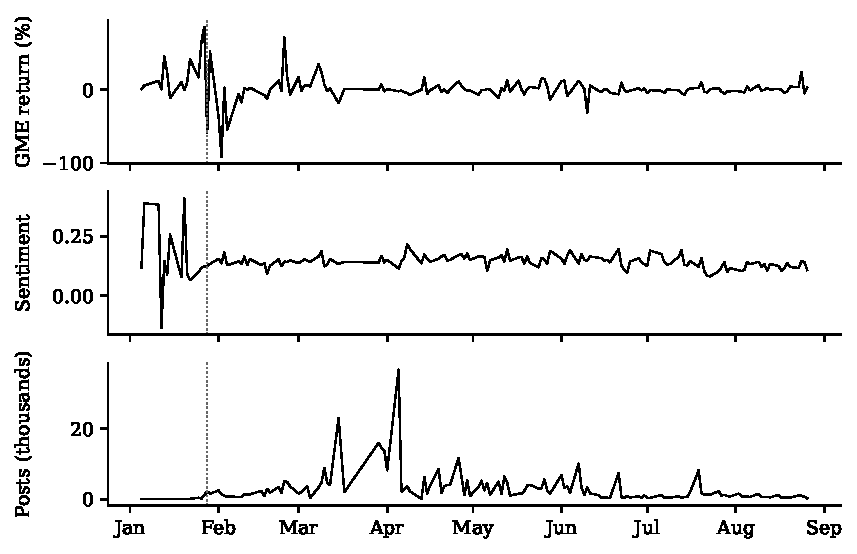
\includegraphics[width=\textwidth]{fig/fig2_revised_panel.pdf}
\caption{GME daily return, Reddit sentiment and number of posts, 5 January --
26 August 2021. Dotted line: 28 January 2021, purchase restrictions by retail
brokers.}
\label{fig:panel}
\end{figure}

\section{Methodology}\label{sec:method}

\paragraph{Replication.} The 2024 specification --- an OLS regression of the GME
closing price on volume, back-filled sentiment and the VIX over 2020--2021 --- is
re-estimated first, to check that the data reproduce the original results.

\paragraph{Stationarity.} Each series is tested with the augmented Dickey--Fuller
test \citep{dickey1979} (null: unit root) and the KPSS test \citep{kpss1992}
(null: stationarity).

\paragraph{Regressions.} Three specifications are estimated with Newey--West
standard errors \citep{newey1987}: (1) a contemporaneous model of returns on
sentiment, the change in attention, the change in volume and the VIX change;
(2) a predictive model of returns on the previous session's sentiment, attention,
return, volume change and VIX change; (3) a model of absolute returns
(volatility) on attention, sentiment and the VIX change. Variance inflation
factors and the condition number check multicollinearity.

\paragraph{Feedback.} Reflexivity implies two-way predictability. Bivariate VARs
with lags chosen by AIC and BIC (maximum 10) are used to test Granger causality
\citep{granger1969} in both directions for sentiment and returns, attention and
returns, and attention and absolute returns.

\paragraph{Wavelet coherence.}\label{sec:wavelet} Wavelet coherence measures the
local correlation between two series across time and periods
\citep{torrence1998,grinsted2004}. I use the Morlet wavelet on periods of 2 to 32
trading days, Monte Carlo significance at 5\% against red-noise benchmarks, and
interpret only results inside the cone of influence. Arrows give the phase:
right means in phase, left anti-phase \citep{aguiar2014}. Sessions without data
are skipped, so the series are treated as consecutive.

\paragraph{Robustness.} The predictive regression and the Granger tests are
re-run excluding the short-squeeze window (11 January -- 5 February 2021), and
the sentiment--return tests over the whole of 2021.

\section{Results}\label{sec:results}

\subsection{Replicating the 2024 results}\label{sec:replication}

The 2024 regression is reproduced almost exactly: on 504 sessions (501 in 2024,
the difference coming from the download date), $R^2=0.820$, $F=761$, a sentiment
coefficient of $-48.2$, a volume coefficient of $-3.2\times10^{-8}$, a VIX
coefficient that is not significant ($p=0.13$), and the same condition number of
$2.7\times10^{8}$. The data are therefore those of the dissertation.

Figure~\ref{fig:replication} shows why these results cannot be interpreted. The
sentiment series is flat at 0.989 for the whole of 2020 --- the value of the two
posts of 4 January 2021, copied backwards --- while the GME price was below US\$5.
From 2021, observed sentiment hovers around 0.15 while the price is ten times
higher. The regression and the $-0.897$ correlation essentially compare these two
regimes: on observed days only, the correlation between sentiment and the price
level falls to $-0.18$. The price level is also non-stationary
(Table~\ref{tab:unitroot}), so a level regression can produce a high $R^2$ without
any economic relationship.

\begin{figure}[htbp]
\centering
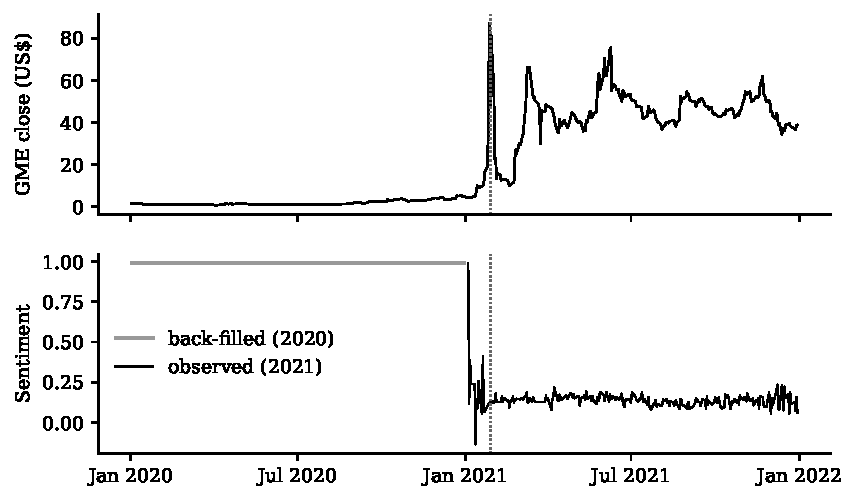
\includegraphics[width=\textwidth]{fig/fig1_replication_series.pdf}
\caption{The 2024 sample: GME closing price and sentiment, 2020--2021. Grey:
values back-filled from the first observed day (4 January 2021); black: observed
values.}
\label{fig:replication}
\end{figure}

\subsection{Descriptive statistics and stationarity}

Table~\ref{tab:desc} describes the revised sample. GME returns are extreme: a
standard deviation of 18\% a day, a kurtosis of 14, and daily log returns between
$-92\%$ and $+85\%$ during the squeeze. Daily sentiment is mildly positive (mean
0.145) and moves little (standard deviation 0.05): post titles are mostly neutral
in VADER terms, and averaging thousands of titles smooths the series further.
Attention is very concentrated, with a median of about 1{,}500 posts per session
and peaks above 36{,}000.

\begin{table}[htbp]
\centering
\caption{Descriptive statistics, 5 January -- 26 August 2021}
\label{tab:desc}
\begin{small}
\begin{tabular}{lrrrrr}
\toprule
 & Return (\%) & Sentiment & Posts & $\Delta\ln$ volume & VIX change (\%) \\
\midrule
Mean & 1.760 & 0.145 & 2,790 & -0.017 & -0.098 \\
Median & -0.013 & 0.142 & 1,459 & -0.060 & -1.212 \\
Std. dev. & 17.995 & 0.051 & 4,308 & 0.691 & 8.951 \\
Min & -91.629 & -0.137 & 2 & -1.798 & -20.840 \\
Max & 85.372 & 0.410 & 36,780 & 3.019 & 48.021 \\
Skewness & 0.234 & 1.283 & 4.586 & 1.156 & 1.233 \\
Kurtosis & 13.623 & 19.539 & 31.859 & 6.230 & 8.731 \\
\bottomrule
\end{tabular}

\end{small}
\par\smallskip\parbox{0.92\textwidth}{\footnotesize Return: daily log return of
GME in percent. Sentiment: post-weighted mean VADER compound score of post
titles. Posts: number of posts per trading session (16 March excluded).
Kurtosis is not excess kurtosis.}
\end{table}

Table~\ref{tab:unitroot} confirms that the GME price level has a unit root, while
returns, sentiment, attention and the changes in volume and VIX are stationary
(sentiment is borderline for KPSS at 5\%). The revised regressors are not
collinear: all variance inflation factors are below 1.2 and the condition number
of the standardised design is 1.5.

\begin{table}[htbp]
\centering
\caption{Unit-root and stationarity tests}
\label{tab:unitroot}
\begin{small}
\begin{tabular}{lrrrr}
\toprule
 & \multicolumn{2}{c}{ADF} & \multicolumn{2}{c}{KPSS} \\
\cmidrule(lr){2-3}\cmidrule(lr){4-5}
Series & stat. & $p$ & stat. & $p$ \\
\midrule
GME close (level) & -0.67 & 0.851 & 3.431 & 0.000 \\
Return & -8.62 & 0.000 & 0.164 & 0.351 \\
Sentiment & -3.53 & 0.007 & 0.524 & 0.035 \\
Attention (log posts) & -4.03 & 0.001 & 0.301 & 0.135 \\
$\Delta\ln$ volume & -10.86 & 0.000 & 0.082 & 0.683 \\
VIX change & -9.22 & 0.000 & 0.086 & 0.657 \\
\bottomrule
\end{tabular}

\end{small}
\par\smallskip\parbox{0.92\textwidth}{\footnotesize GME close: log price over
2020--2021. Other series: main sample. ADF: null of a unit root (lag length by
AIC). KPSS: null of stationarity. Constant included.}
\end{table}

\subsection{Sentiment, attention and returns}

Table~\ref{tab:reg} reports the regressions. In the contemporaneous model
(column 1), sentiment has no relationship with same-day returns ($-8.7$,
$p=0.58$), nor does the change in attention. Trading volume is the only
significant variable: a doubling of volume (a log change of 0.69) is associated
with a return about 4.7 percentage points higher ($6.85$, $p=0.008$). The model
explains 16\% of daily return variance, largely through volume.

The predictive model (column 2) is where the 2024 intuition finds some support,
though not in the expected direction. Higher sentiment and higher attention on
one day are followed by \emph{lower} returns the next day: a one-standard-deviation
rise in sentiment (0.05) predicts a return about 2.7 points lower ($-53.4$,
$p=0.006$), and a 1\% increase in posts a return 0.019 points lower
($-1.88$, $p=0.008$). This is a reversal pattern --- euphoria followed by
correction --- consistent with attention-driven price pressure that later unwinds
\citep{da2011}.

This result, however, belongs to the squeeze. Excluding 11 January -- 5 February
2021, the lagged sentiment coefficient falls to $-30.0$ and becomes insignificant
($p=0.35$), and the attention coefficient turns positive and insignificant
($p=0.47$); only a small positive autocorrelation of returns remains. Over the
whole of 2021, lagged sentiment is negative but only marginally significant
($-32.0$, $p=0.075$). In January, moreover, sentiment is computed on very few
posts, which makes the series noisy exactly when returns are most extreme.

Column 3 shows that attention and sentiment do not explain the size of daily
moves ($R^2=0.003$). The correlation between attention and absolute returns is
0.78 over the fifteen sessions up to and including 28 January, but only 0.15
afterwards.

\begin{table}[htbp]
\centering
\caption{GME returns, sentiment and attention}
\label{tab:reg}
\begin{small}
\begin{tabular}{lccc}
\toprule
 & (1) Return$_t$ & (2) Return$_t$ & (3) $|$Return$_t|$ \\
 & contemporaneous & predictive & attention \\
\midrule
Constant & $3.124$ & $22.533^{***}$ & $12.371$ \\
 & $(3.452)$ & $(7.313)$ & $(7.905)$ \\
Sentiment$_t$ & $-8.740$ &  & $-12.736$ \\
 & $(15.628)$ &  & $(23.701)$ \\
$\Delta$ attention$_t$ & $0.208$ &  &  \\
 & $(0.888)$ &  &  \\
$\Delta\ln$ volume$_t$ & $6.846^{***}$ &  &  \\
 & $(2.568)$ &  &  \\
VIX change$_t$ & $0.641$ &  & $0.057$ \\
 & $(0.453)$ &  & $(0.254)$ \\
Sentiment$_{t-1}$ &  & $-53.440^{***}$ &  \\
 &  & $(19.424)$ &  \\
Attention$_{t-1}$ &  & $-1.882^{***}$ &  \\
 &  & $(0.711)$ &  \\
Return$_{t-1}$ &  & $0.110$ &  \\
 &  & $(0.092)$ &  \\
$\Delta\ln$ volume$_{t-1}$ &  & $0.390$ &  \\
 &  & $(1.783)$ &  \\
VIX change$_{t-1}$ &  & $-0.414$ &  \\
 &  & $(0.268)$ &  \\
Attention$_t$ (log posts) &  &  & $-0.200$ \\
 &  &  & $(0.621)$ \\
\midrule
$R^2$ & 0.160 & 0.099 & 0.003 \\
Observations & 146 & 150 & 151 \\
\bottomrule
\end{tabular}

\end{small}
\par\smallskip\parbox{0.92\textwidth}{\footnotesize Main sample. Returns and VIX
change in percent. Attention: log number of posts. Newey--West standard errors (5
lags) in parentheses; $^{*}$, $^{**}$, $^{***}$: significance at 10\%, 5\%, 1\%.}
\end{table}

\subsection{Testing for feedback}

Table~\ref{tab:granger} reports the Granger tests. Sentiment helps forecast
returns when eight lags are allowed ($p<0.001$), but not with the single lag
chosen by the BIC ($p=0.097$). In the other direction, returns never help
forecast sentiment ($p=0.27$ and $0.54$). Attention helps forecast absolute
returns ($p=0.008$ with five lags, $0.061$ with two), but absolute returns do not
forecast attention, and attention does not forecast the sign of returns.

Two findings follow. First, there is no evidence of the \emph{two-way} loop that
reflexivity implies: whatever predictability exists runs from Reddit to prices,
not back. Second, the one-way predictability is again a squeeze phenomenon:
excluding 11 January -- 5 February 2021, none of the tests is significant (all
$p>0.28$). Over the whole of 2021, sentiment Granger-causes returns at four lags
($p=0.023$), and returns still do not Granger-cause sentiment ($p=0.27$).

\begin{table}[htbp]
\centering
\caption{Granger causality tests}
\label{tab:granger}
\begin{small}
\begin{tabular}{lcccc}
\toprule
 & \multicolumn{2}{c}{Lag selected by AIC} & \multicolumn{2}{c}{Lag selected by BIC} \\
\cmidrule(lr){2-3}\cmidrule(lr){4-5}
Null hypothesis & lag, $F$ & $p$ & lag, $F$ & $p$ \\
\midrule
Sentiment $\nrightarrow$ Return & 8, 5.90 & 0.000 & 1, 2.80 & 0.097 \\
Return $\nrightarrow$ Sentiment & 8, 1.26 & 0.271 & 1, 0.38 & 0.541 \\
Attention $\nrightarrow$ Return & 4, 1.85 & 0.124 & 4, 1.85 & 0.124 \\
Return $\nrightarrow$ Attention & 4, 1.94 & 0.107 & 4, 1.94 & 0.107 \\
Attention $\nrightarrow$ $|$Return$|$ & 5, 3.24 & 0.008 & 2, 2.85 & 0.061 \\
$|$Return$|$ $\nrightarrow$ Attention & 5, 0.77 & 0.570 & 2, 0.52 & 0.598 \\
\bottomrule
\end{tabular}

\end{small}
\par\smallskip\parbox{0.92\textwidth}{\footnotesize $X \nrightarrow Y$: null
hypothesis that $X$ does not Granger-cause $Y$. $F$-tests from bivariate VARs,
maximum lag 10. Main sample.}
\end{table}

\subsection{Wavelet coherence}

Figure~\ref{fig:wtcsr} shows the wavelet coherence between sentiment and returns.
Only 0.9\% of the time--frequency plane inside the cone of influence is
significant at 5\% --- less than the 5\% expected by chance. There is no
time-frequency band in which daily sentiment and returns move together. Between
attention and absolute returns (Figure~\ref{fig:wtcav}), 5.2\% of the plane is
significant, about what chance would produce; the significant islands are short
(2--8 trading days), scattered between March and July, and without a dominant
phase.

\begin{figure}[htbp]
\centering
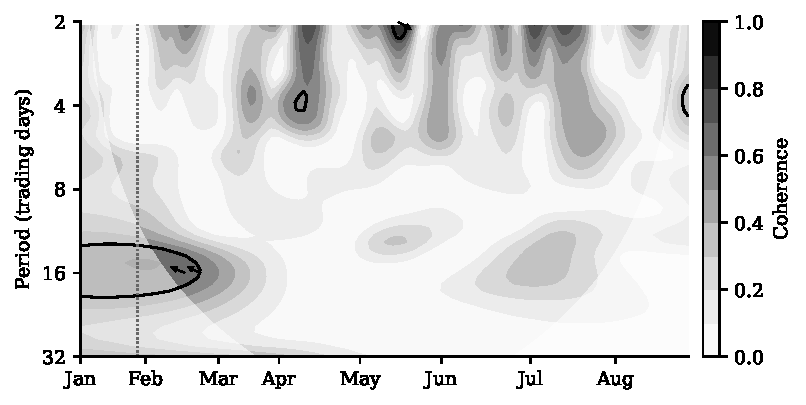
\includegraphics[width=\textwidth]{fig/fig3_wtc_sent_ret.pdf}
\caption{Wavelet coherence between Reddit sentiment and GME returns. Thick
contours: 5\% significance; hatched: outside the cone of influence; dotted line:
28 January 2021.}
\label{fig:wtcsr}
\end{figure}

\begin{figure}[htbp]
\centering
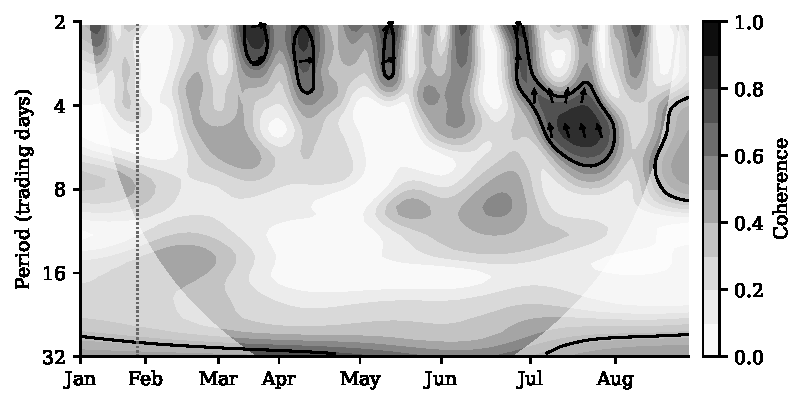
\includegraphics[width=\textwidth]{fig/fig4_wtc_att_vol.pdf}
\caption{Wavelet coherence between attention (log posts) and absolute GME returns.}
\label{fig:wtcav}
\end{figure}

\section{Discussion}

\subsection{Interpretation}

The results do not support H1 as formulated: daily Reddit data show no feedback
from prices to sentiment, and no coherent co-movement between the two. H2 holds
only in a limited and unexpected form: during the squeeze, higher sentiment and
attention preceded \emph{lower} next-day returns, a reversal rather than a
self-reinforcing rally. H3 receives the clearest support: trading volume moves
strongly with returns, and online attention preceded volatility in the weeks
around 28 January 2021.

Read through Soros's lens, the picture is that of a short reflexive episode
rather than a persistent mechanism. In January 2021, attention, trading and
prices did reinforce each other; once the brokers' restrictions broke the
episode, Reddit activity no longer told much about GME prices. This is close to
the attention literature \citep{barber2008,da2011}: what moved prices was the
intensity of retail activity, not the tone of what retail investors wrote.

\subsection{Alternative explanations and limits}

\begin{itemize}
\item \textbf{Measurement.} VADER scores of post titles capture tone poorly on
WallStreetBets-style language (slang, irony, emojis), and daily averages of
thousands of titles leave little variation. A finance-specific model would
measure sentiment better.
\item \textbf{Frequency.} Feedback between posts and prices may operate within the
day, which daily data cannot see.
\item \textbf{Data.} The Reddit file is truncated and contains a collection
artefact; early January is thinly covered, precisely when the squeeze started.
\item \textbf{Common drivers.} Media coverage, options activity and institutional
positioning may have moved both Reddit activity and prices, as the 2024 edition
already noted; the tests used here measure predictability, not causality.
\end{itemize}

\section{Comparison with the 2024 edition}\label{sec:compare}

\begin{small}
\begin{tabular}{@{}L{0.22\textwidth}L{0.34\textwidth}L{0.38\textwidth}@{}}
\toprule
Point & 2024 edition & Revised analysis (2026) \\
\midrule
Sample & 501 days, Jan 2020 -- Dec 2021 & 151 sessions, 5 Jan -- 26 Aug 2021
(days with Reddit data) \\[2pt]
Sentiment & Mean 0.565, median 0.989 & Mean 0.145, s.d. 0.05 (2020 values
were back-filled) \\[2pt]
Sentiment--price link & Correlation $-0.897$; OLS $R^2=0.82$ & Artefact of the
back-fill and of price levels; no same-day link with returns \\[2pt]
Sentiment as leading indicator & Asserted from the wavelet heatmap & Lagged
sentiment predicts lower returns, only during the squeeze \\[2pt]
Reflexive feedback & Supported & Not found: returns never predict sentiment \\[2pt]
Volume & Small negative effect on price level & Strong positive association
with same-day returns \\[2pt]
Wavelet coherence & Higher at low frequencies & Not significant for sentiment;
chance level for attention \\[2pt]
Main message & Reflexivity and sentiment drive meme stocks & Attention and
trading, not sentiment tone, accompanied a short reflexive episode in January
2021 \\
\bottomrule
\end{tabular}
\end{small}

\section{Recommendations}

\paragraph{Investors.} Reddit sentiment is not a reliable trading signal for GME
outside the squeeze, and during the squeeze it pointed to reversals. Attention and
volume are better warning signs of risk than of returns; in such conditions,
position limits and stop-losses matter more than sentiment indicators.

\paragraph{Companies.} Firms at the centre of retail attention should expect
volatility to follow surges in online activity, and benefit from clear and timely
communication when attention spikes.

\paragraph{Regulators.} Monitoring retail attention --- post volumes, new
accounts, options activity --- seems more useful than monitoring tone. The
financial-education recommendation of the 2024 edition stands: the speed at
which attention-driven episodes form and unwind is precisely what inexperienced
investors underestimate.

\paragraph{Research.} Natural extensions are intraday data, a finance-specific
sentiment model, the complete Reddit archive, comparison with other meme stocks
(AMC) and with non-meme peers, and an event-study design around the 28 January
restrictions.

\section{Conclusion}

This dissertation set out to test whether reflexivity and Reddit sentiment
explain meme-stock prices. The original answer --- a strong, sentiment-driven
reflexive dynamic --- rested on an artefact of data construction. With the data
that actually exist, the answer is narrower and more precise. Daily sentiment did
not move with GameStop's returns, and prices did not feed back into sentiment;
the predictive content of sentiment and attention was concentrated in the few
weeks of the January 2021 squeeze, and it pointed to reversals. Trading volume
and the intensity of online attention, rather than the tone of posts, are the
measurable traces of retail influence. Reflexivity may well describe what
happened in January 2021, but it was a brief episode, not a lasting regime.

\section*{Reproducibility}
\addcontentsline{toc}{section}{Reproducibility}

All tables and figures are produced by \texttt{revised\_analysis.py} (Python 3,
with pandas, statsmodels, arch, pycwt, matplotlib and yfinance) from
\texttt{data/daily\_reddit\_sentiment.csv} and the GME and VIX series cached in
\texttt{gme\_vix\_daily.csv}. The Monte Carlo significance of the wavelet
coherence uses a fixed random seed.

\begin{thebibliography}{99}
\setlength{\itemsep}{1pt}\small

\bibitem[Aguiar-Conraria and Soares(2014)]{aguiar2014}
Aguiar-Conraria, L. and Soares, M. J. (2014). The continuous wavelet transform:
moving beyond uni- and bivariate analysis. \emph{Journal of Economic Surveys},
28(2), 344--375.

\bibitem[Antweiler and Frank(2004)]{antweiler2004}
Antweiler, W. and Frank, M. Z. (2004). Is all that talk just noise? The
information content of internet stock message boards. \emph{Journal of Finance},
59(3), 1259--1294.

\bibitem[Barber and Odean(2008)]{barber2008}
Barber, B. M. and Odean, T. (2008). All that glitters: the effect of attention
and news on the buying behavior of individual and institutional investors.
\emph{Review of Financial Studies}, 21(2), 785--818.

\bibitem[Betzer and Harries(2022)]{betzer2022}
Betzer, A. and Harries, J. P. (2022). How online discussion board activity
affects stock trading: the case of GameStop. \emph{Financial Markets and Portfolio
Management}, 36(4), 443--472.

\bibitem[Da et~al.(2011)]{da2011}
Da, Z., Engelberg, J. and Gao, P. (2011). In search of attention. \emph{Journal of
Finance}, 66(5), 1461--1499.

\bibitem[Dickey and Fuller(1979)]{dickey1979}
Dickey, D. A. and Fuller, W. A. (1979). Distribution of the estimators for
autoregressive time series with a unit root. \emph{Journal of the American
Statistical Association}, 74(366), 427--431.

\bibitem[Garvey et~al.(2023)]{garvey2023}
Garvey, R., He, J. and Wu, F. (2023). Retail broker trading restrictions and
market liquidity: an examination of GameStop. \emph{Applied Economics}, 56(34),
4140--4153.

\bibitem[Graham(1949)]{graham1949}
Graham, B. (1949). \emph{The Intelligent Investor}. Harper \& Brothers.

\bibitem[Granger(1969)]{granger1969}
Granger, C. W. J. (1969). Investigating causal relations by econometric models
and cross-spectral methods. \emph{Econometrica}, 37(3), 424--438.

\bibitem[Grinsted et~al.(2004)]{grinsted2004}
Grinsted, A., Moore, J. C. and Jevrejeva, S. (2004). Application of the cross
wavelet transform and wavelet coherence to geophysical time series.
\emph{Nonlinear Processes in Geophysics}, 11, 561--566.

\bibitem[Han and Iliadis(2023)]{han2023}
Han, J. and Iliadis, A. (2023). \emph{GameStop Reddit Dataset}. Temple
University. Public domain.

\bibitem[Hutto and Gilbert(2014)]{hutto2014}
Hutto, C. J. and Gilbert, E. (2014). VADER: a parsimonious rule-based model for
sentiment analysis of social media text. \emph{Proceedings of the International
AAAI Conference on Web and Social Media}, 8(1), 216--225.

\bibitem[Kwiatkowski et~al.(1992)]{kpss1992}
Kwiatkowski, D., Phillips, P. C. B., Schmidt, P. and Shin, Y. (1992). Testing
the null hypothesis of stationarity against the alternative of a unit root.
\emph{Journal of Econometrics}, 54(1--3), 159--178.

\bibitem[Long et~al.(2022)]{long2022}
Long, S. C., Lucey, B., Xie, Y. and Yarovaya, L. (2022). ``I just like the
stock'': the role of Reddit sentiment in GameStop. Working paper, SSRN.

\bibitem[Malz(2021)]{malz2021}
Malz, A. M. (2021). The GameStop episode: what happened and what does it mean?
\emph{Cato Journal}, 41(3).

\bibitem[Newey and West(1987)]{newey1987}
Newey, W. K. and West, K. D. (1987). A simple, positive semi-definite,
heteroskedasticity and autocorrelation consistent covariance matrix.
\emph{Econometrica}, 55(3), 703--708.

\bibitem[Soros(1987)]{soros1987}
Soros, G. (1987). \emph{The Alchemy of Finance}. Simon \& Schuster.

\bibitem[Soros(1998)]{soros1998}
Soros, G. (1998). \emph{The Crisis of Global Capitalism: Open Society
Endangered}. PublicAffairs.

\bibitem[Tetlock(2007)]{tetlock2007}
Tetlock, P. C. (2007). Giving content to investor sentiment: the role of media in
the stock market. \emph{Journal of Finance}, 62(3), 1139--1168.

\bibitem[Torrence and Compo(1998)]{torrence1998}
Torrence, C. and Compo, G. P. (1998). A practical guide to wavelet analysis.
\emph{Bulletin of the American Meteorological Society}, 79(1), 61--78.

\bibitem[Umar et~al.(2021)]{umar2021}
Umar, Z., Gubareva, M., Yousaf, I. and Ali, S. (2021). A tale of company
fundamentals vs sentiment-driven pricing: the case of GameStop. \emph{Journal of
Behavioral and Experimental Finance}, 30, 100501.

\end{thebibliography}

\subsection*{Other sources cited in the 2024 edition}
{\small
\begin{itemize}[leftmargin=*]
\item Crouhy, M., Galai, D. and Mark, R. (2006). \emph{The Essentials of Risk
Management}. McGraw-Hill.
\item De Silva, T., So, E. C. and Smith, K. (2024). Losing is optional: retail
option trading and expected announcement volatility. Working paper, MIT.
\item Gao, J. (2022). Analysis of the impact on GameStop from the GameStop
opportunistic episode. \emph{Journal of Education, Humanities and Social
Sciences}, 2, 186--192.
\item Grundmann, L. (2021). From lambs to lions: how did retail investors' role
and trading behavior change in the light of WallStreetBets? Thesis.
\item Han, S. (2024). Unveiling the sophistication: understanding retail
investors' trading behavior in the U.S. options market. Cboe Global Markets.
\item Li, Y., Zhao, C. and Zhong, Z. (2021). Trading behavior of retail investors
in derivatives markets: evidence from Mini options. \emph{Journal of Banking \&
Finance}, 133, 106250.
\item Markoch, C. (2024). GameStop stock is giving investors a familiar feeling,
but why? MarketBeat, 12 March 2024.
\item Mishra, Kumar and Biraj (2016). Classification of retail investors: a
behavioural study. \emph{International Journal of Applied Business and Economic
Research}.
\item Simpson, A. (2023). From Main Street to Wall Street: analysis of retail
trading power after the GameStop squeeze. \emph{Journal of Student Research},
12(4).
\item \emph{To the moon: analyzing collective trading events on the wings of
sentiment analysis} (2023). ResearchGate.
\item Wang, K., Wong, B., Khoshkholghi, M. A., Shah, P., Naha, R., Mahanti, A.
and Kim, J. (2024). Dissecting the hype: a study of WallStreetBets' sentiment and
network correlation on financial markets. \emph{Lecture Notes on Data Engineering
and Communications Technologies}, 263--273.
\end{itemize}
}

\end{document}
